%!TEX program = xelatex
% not lualatex because of a pgf bug: https://sourceforge.net/p/pgf/bugs/384/
\documentclass[12pt, a4paper]{report}
\usepackage[T1]{fontenc}
\usepackage[english]{babel}
\usepackage[colorlinks=true, linkcolor=red, urlcolor=]{hyperref}
\usepackage{utbmcovers}
\usepackage{titlesec}
\usepackage[nottoc]{tocbibind}
\usepackage{graphicx}
\usepackage{subfig}
\usepackage[acronym]{glossaries}

\titleformat{\chapter}[block]{\normalfont\huge\bfseries}{\thechapter.}{5pt}{\Huge}
\titlespacing{\chapter}{0pt}{0pt}{40pt}
\setcounter{tocdepth}{0} % Show chapters only
\newfontfamily\italictahomafont{Tahoma}[FakeSlant=0.4]
\graphicspath{ {images/} }
\renewcommand*{\glstextformat}[1]{\textcolor{black}{#1}}

%----------------------------------------
% utbmcovers configuration
%----------------------------------------
\setutbmfrontillustration{report_cover}
\setutbmtitle{Deep Learning for Egocentric vision}
\setutbmsubtitle{ST50 thesis - P2020}
\setutbmstudent{GUETARNI Bilel}
\setutbmstudentdepartment{Computer Science department}
\setutbmstudentpathway{Image, Interaction et Réalité Virtuelle}
\setutbmcompany{Haute Ecole d'Ingénierie et de Gestion du Canton de Vaud}
\setutbmcompanyaddress{Avenue des Sports 29\\1400 Yverdon-les-Bains}
\setutbmcompanywebsite{\href{https://heig-vd.ch/}{heig-vd.ch}}
\setutbmcompanytutor{PEREZ-URIBE Andres}
\setutbmschooltutor{GABER Jaafar}
\setutbmkeywords{Deep Learning - Computer vision - Action recognition - Egocentric vision - GPU - Patient follow-up}
\setutbmabstract{
	Deep learning has been widely used in computer vision in the last two decades.
	Several tasks have been addressed with, including object detection, content generation, image or instance segmentation and a couple of others.
	Nowadays very complex tasks are at the heart of academic research, including action/activity recognition; these two last are really similar, the difference is slight so here we will use the term of action recognition (the difference can be for example the action of picking a fork during the activity of cooking).
	Particularly, achieving action recognition at a reasonable accuracy could allow the follow-up of people with reduced physical capacities especially with tremors in their daily life.
	It will be then easy to identify the actions that a person struggle with, and then conduct a targeted rehabilitation process.
	In this internship I explored how deep learning can be applied in this particular task and what the actual state-of-the-art is.
	I focused on cheap computation solutions as it is expected to be used on edge devices; e.g. mobile phone, embedded device...
}

\makeglossaries
\newglossaryentry{ego}
{
    name=Egocentric view,
    description={first person view}
}
\newglossaryentry{nlp}
{
    name=Natural Language Processing,
    description={automatic process of language by computer}
}
\newglossaryentry{synthdata}
{
    name=Synthetic-to-Real domain gap,
    description={the unreal property of synthetic data that impacts models accuracy when trained on}
}
\begin{document}
	\makeutbmfrontcover{}

	% write table of content
	{
	\hypersetup{linkcolor=black}
	\tableofcontents
	}
	
	% write acronyms
	\printglossary
	
	\chapter{Introduction}
	\section{Deep Learning and Computer Vision}
	Deep Learning is a really successful field that is currently under innumerable investigations.
	Despite the well-known difficulties associated, numerous people jump into it every day.
	It has been successfully applied to several domains like Computer Vision, \gls{nlp}, board games and a raft of others.
	The first one is currently the most explored with a lot of academic research associated with huge industrial applications.
	Deep learning has revolutionized the field of computer vision by its accuracy never reached by classical algorithms.
	From the beginning, computer vision played an important role in the development of deep learning \cite{lecun_zipcode,lecun_mnist}.
	Today, it's a popular opinion that among the roads to explore to resolve a problem, deep learning is a major one.\\
	However, it suffers from a major drawback, its need of enormous datasets.
	As the tasks tackled become more and more complex, the systems need more and more data to reach an acceptable accuracy.
	Also, most systems for computer vision are trained in a supervised learning fashion which requires data to be labeled, and for some tasks it is really hard to find such ones (even if synthetic data can be used, this still raise the problem of \gls{synthdata}).
	Moreover, the more data we have, the more computations are then needed, and we know that recent deep learning systems can take several weeks to train.\\
	
	Despite those drawbacks, and because several workarounds have been developed, deep learning is still seen as a powerful tool to enhance our systems.

	\section{Action recognition}
	Content recognition is at the heart of the literature since the beginning. It began with numbers \cite{lecun_mnist}, animals (e.g. cats for the most popular one) and more recently complex concepts as actions.
	Human action recognition requires developing systems that can capture motion over time, for sequence prediction, or systems that recognize an action through a single frame.
	The first case has seen emerged novels architecture as 3D convolutional networks \cite{3dcnn} and two-stream architectures (see \ref{twostream}).
	It is worth to notice that action recognition is itself split in two categories: first person view, also known as \gls{ego} (Figure \ref{f1}), and third person view (Figure \ref{f2}); in this work, we focus on egocentric view action recognition.
	If we look in the literature, we'll see that egocentric vision has been neglected over third person view.
	Nonetheless, large scaled recently published datasets have exposed the egocentric view problematic and encouraged research for.\\
	\begin{figure}[!tbp]
		\centering
		\subfloat[First person.]{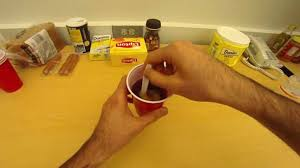
\includegraphics[width=0.4\textwidth]{firstperson.jpeg}\label{f1}}
		\hfill
		\subfloat[Third person.]{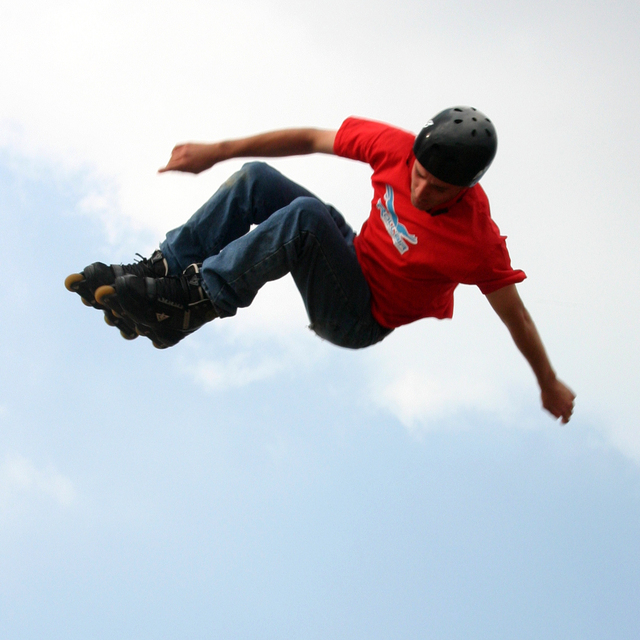
\includegraphics[width=0.4\textwidth]{thirdperson.jpg}\label{f2}}
		\caption{Action views.}
	\end{figure}
	Among the different applications of action recognition we find patient follow-up.
	Medical stuff could use automatic egocentric view action recognition to find which actions in the daily-life of a person with physical abilities disorders are the most difficult for them\footnote{Of course recognize the action is not sufficient, one should detect the disorders.}.
	And then use these analyses to conduct a targeted rehabilitation process.\\
	Another task that is similar and increasingly covered is image captioning \cite{imagecaption}, where a model try to add a caption to an image; which is highly related to scene understanding.
	It is easy to see that they are sensibly similar and actually, many advances that came out for image captioning are now used for action recognition (attention mechanism, recurrent).


	\chapter{State-of-the-art}
	\section{Two-stream architectures}\label{twostream}
	Lorem ipsu.

	\section{EPIC-KITCHENS}
	Lorem ipsu.

	\bibliographystyle{unsrt}
	\bibliography{bibliography}
	\makeutbmbackcover{}
\end{document}
